% =====================================================================
% Section 4 — Results
% =====================================================================
% All numerical values in this section are taken from the dissertation
% \citep{porto2026dissertation} and the associated sizing notes
% for the intake valve and the valve springs of the AP 1.8 head. No
% value is invented; every figure traces to a source.
% =====================================================================

\section{Results}\label{sec:results}

\subsection{Populated BowTie diagram}\label{sec:res-bowtie}

Figure~\ref{fig:bowtie} shows the populated BowTie diagram for the AP
1.8 valve train at 10\,000~rpm, around the top event \emph{loss of
follower contact between valve and cam}. The threats, preventive
barriers, consequences, and mitigative barriers are those of
Section~\ref{sec:method-bowtie-qual}.

% =====================================================================
% Figure 1 — BowTie diagram (TikZ-generated)
% =====================================================================

\begin{figure*}[t]
  \centering
  % =====================================================================
% Figure 1 — BowTie diagram (TikZ-native)
%
% Generated as vector graphics inside the document; no external file
% needed. Loaded into Section 4 via % =====================================================================
% Figure 1 — BowTie diagram (TikZ-native)
%
% Generated as vector graphics inside the document; no external file
% needed. Loaded into Section 4 via % =====================================================================
% Figure 1 — BowTie diagram (TikZ-native)
%
% Generated as vector graphics inside the document; no external file
% needed. Loaded into Section 4 via \input{figs/fig1_bowtie.tex}.
% =====================================================================

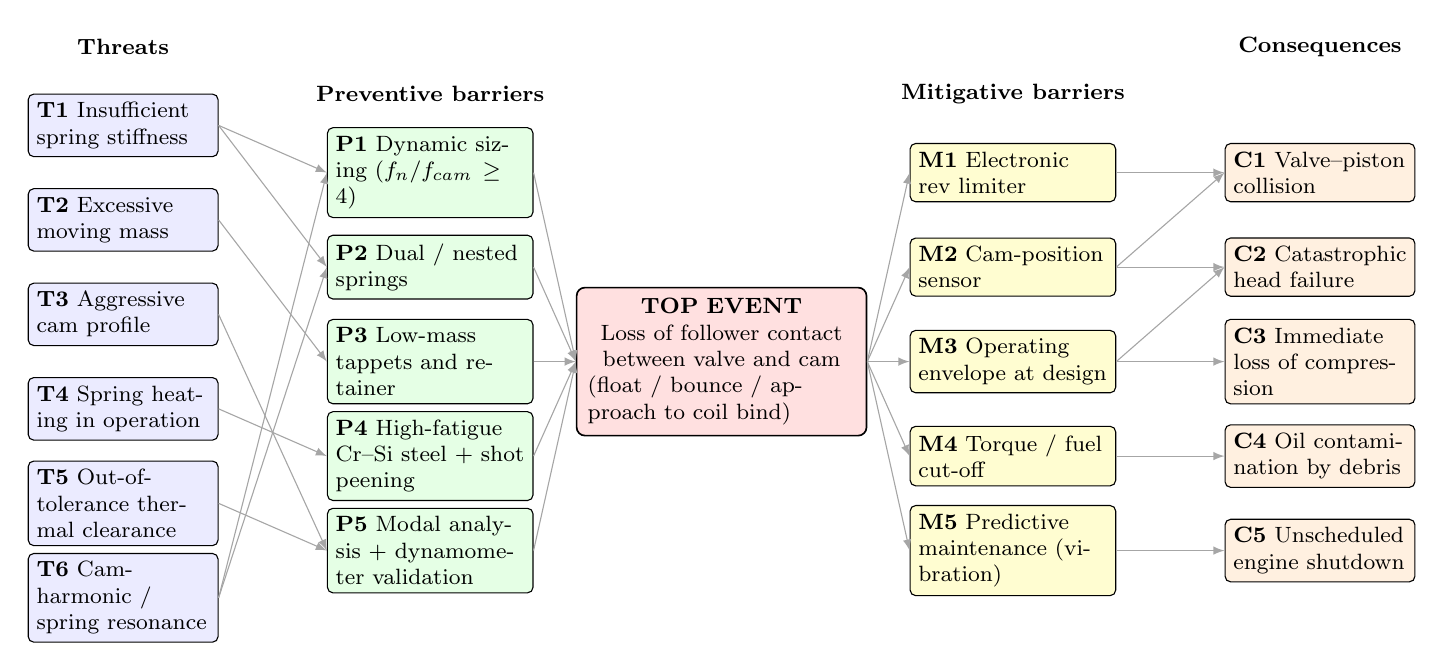
\begin{tikzpicture}[
  font=\footnotesize,
  every node/.style={align=left},
  threat/.style={draw,fill=blue!8,rounded corners=2pt,inner sep=3pt,minimum width=22mm,minimum height=6mm,text width=22mm},
  pbar/.style={draw,fill=green!10,rounded corners=2pt,inner sep=3pt,minimum width=24mm,minimum height=6mm,text width=24mm},
  cons/.style={draw,fill=orange!12,rounded corners=2pt,inner sep=3pt,minimum width=22mm,minimum height=6mm,text width=22mm},
  mbar/.style={draw,fill=yellow!18,rounded corners=2pt,inner sep=3pt,minimum width=24mm,minimum height=6mm,text width=24mm},
  topev/.style={draw,fill=red!12,line width=0.6pt,rounded corners=3pt,inner sep=4pt,minimum width=34mm,minimum height=12mm,text width=34mm},
  flow/.style={->,>=latex,line width=0.4pt,gray!70},
]

% ---- Top event (centre)
\node[topev] (TE) at (0,0)
  {\centering\textbf{TOP EVENT}\\Loss of follower contact between valve and cam\\(float / bounce / approach to coil bind)};

% ---- Threats (left, T1..T6)
\node[threat] (T1) at (-7.6, 3.0) {\textbf{T1} Insufficient spring stiffness};
\node[threat] (T2) at (-7.6, 1.8) {\textbf{T2} Excessive moving mass};
\node[threat] (T3) at (-7.6, 0.6) {\textbf{T3} Aggressive cam profile};
\node[threat] (T4) at (-7.6,-0.6) {\textbf{T4} Spring heating in operation};
\node[threat] (T5) at (-7.6,-1.8) {\textbf{T5} Out-of-tolerance thermal clearance};
\node[threat] (T6) at (-7.6,-3.0) {\textbf{T6} Cam-harmonic / spring resonance};

% ---- Preventive barriers (between threats and TE)
\node[pbar] (P1) at (-3.7, 2.4) {\textbf{P1} Dynamic sizing ($f_n/f_{cam}\geq 4$)};
\node[pbar] (P2) at (-3.7, 1.2) {\textbf{P2} Dual / nested springs};
\node[pbar] (P3) at (-3.7, 0.0) {\textbf{P3} Low-mass tappets and retainer};
\node[pbar] (P4) at (-3.7,-1.2) {\textbf{P4} High-fatigue Cr--Si steel + shot peening};
\node[pbar] (P5) at (-3.7,-2.4) {\textbf{P5} Modal analysis + dynamometer validation};

% ---- Consequences (right, C1..C5)
\node[cons] (C1) at (7.6, 2.4) {\textbf{C1} Valve--piston collision};
\node[cons] (C2) at (7.6, 1.2) {\textbf{C2} Catastrophic head failure};
\node[cons] (C3) at (7.6, 0.0) {\textbf{C3} Immediate loss of compression};
\node[cons] (C4) at (7.6,-1.2) {\textbf{C4} Oil contamination by debris};
\node[cons] (C5) at (7.6,-2.4) {\textbf{C5} Unscheduled engine shutdown};

% ---- Mitigative barriers (between TE and consequences)
\node[mbar] (M1) at (3.7, 2.4) {\textbf{M1} Electronic rev limiter};
\node[mbar] (M2) at (3.7, 1.2) {\textbf{M2} Cam-position sensor};
\node[mbar] (M3) at (3.7, 0.0) {\textbf{M3} Operating envelope at design};
\node[mbar] (M4) at (3.7,-1.2) {\textbf{M4} Torque / fuel cut-off};
\node[mbar] (M5) at (3.7,-2.4) {\textbf{M5} Predictive maintenance (vibration)};

% ---- Threats -> Preventive barriers (many-to-some mapping)
\draw[flow] (T1.east) -- (P1.west);
\draw[flow] (T2.east) -- (P3.west);
\draw[flow] (T3.east) -- (P5.west);
\draw[flow] (T4.east) -- (P4.west);
\draw[flow] (T5.east) -- (P5.west);
\draw[flow] (T6.east) -- (P1.west);
\draw[flow] (T1.east) -- (P2.west);
\draw[flow] (T6.east) -- (P2.west);

% ---- Preventive barriers -> Top event
\draw[flow] (P1.east) -- (TE.west);
\draw[flow] (P2.east) -- (TE.west);
\draw[flow] (P3.east) -- (TE.west);
\draw[flow] (P4.east) -- (TE.west);
\draw[flow] (P5.east) -- (TE.west);

% ---- Top event -> Mitigative barriers
\draw[flow] (TE.east) -- (M1.west);
\draw[flow] (TE.east) -- (M2.west);
\draw[flow] (TE.east) -- (M3.west);
\draw[flow] (TE.east) -- (M4.west);
\draw[flow] (TE.east) -- (M5.west);

% ---- Mitigative barriers -> Consequences
\draw[flow] (M1.east) -- (C1.west);
\draw[flow] (M2.east) -- (C1.west);
\draw[flow] (M3.east) -- (C2.west);
\draw[flow] (M3.east) -- (C3.west);
\draw[flow] (M4.east) -- (C4.west);
\draw[flow] (M5.east) -- (C5.west);
\draw[flow] (M2.east) -- (C2.west);

% ---- Side labels
\node[font=\footnotesize\bfseries] at (-7.6, 4.0) {Threats};
\node[font=\footnotesize\bfseries] at (-3.7, 3.4) {Preventive barriers};
\node[font=\footnotesize\bfseries] at ( 3.7, 3.4) {Mitigative barriers};
\node[font=\footnotesize\bfseries] at ( 7.6, 4.0) {Consequences};

\end{tikzpicture}
.
% =====================================================================

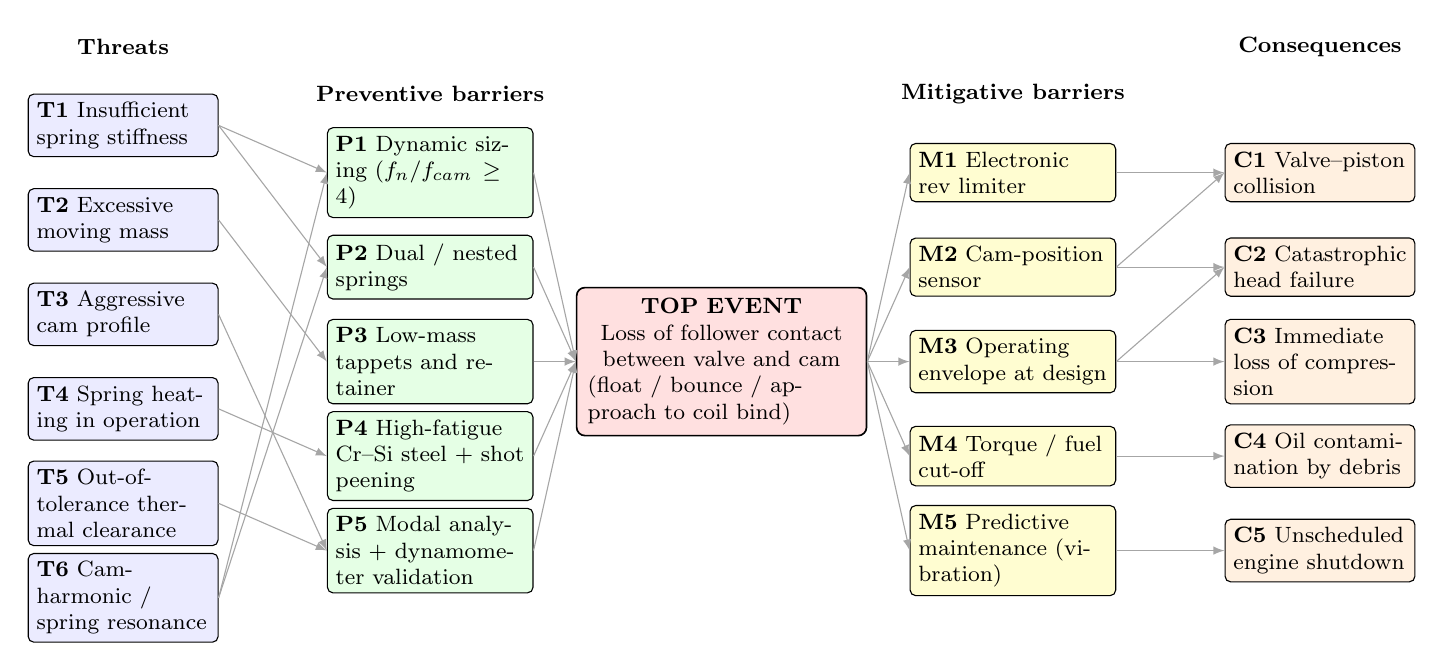
\begin{tikzpicture}[
  font=\footnotesize,
  every node/.style={align=left},
  threat/.style={draw,fill=blue!8,rounded corners=2pt,inner sep=3pt,minimum width=22mm,minimum height=6mm,text width=22mm},
  pbar/.style={draw,fill=green!10,rounded corners=2pt,inner sep=3pt,minimum width=24mm,minimum height=6mm,text width=24mm},
  cons/.style={draw,fill=orange!12,rounded corners=2pt,inner sep=3pt,minimum width=22mm,minimum height=6mm,text width=22mm},
  mbar/.style={draw,fill=yellow!18,rounded corners=2pt,inner sep=3pt,minimum width=24mm,minimum height=6mm,text width=24mm},
  topev/.style={draw,fill=red!12,line width=0.6pt,rounded corners=3pt,inner sep=4pt,minimum width=34mm,minimum height=12mm,text width=34mm},
  flow/.style={->,>=latex,line width=0.4pt,gray!70},
]

% ---- Top event (centre)
\node[topev] (TE) at (0,0)
  {\centering\textbf{TOP EVENT}\\Loss of follower contact between valve and cam\\(float / bounce / approach to coil bind)};

% ---- Threats (left, T1..T6)
\node[threat] (T1) at (-7.6, 3.0) {\textbf{T1} Insufficient spring stiffness};
\node[threat] (T2) at (-7.6, 1.8) {\textbf{T2} Excessive moving mass};
\node[threat] (T3) at (-7.6, 0.6) {\textbf{T3} Aggressive cam profile};
\node[threat] (T4) at (-7.6,-0.6) {\textbf{T4} Spring heating in operation};
\node[threat] (T5) at (-7.6,-1.8) {\textbf{T5} Out-of-tolerance thermal clearance};
\node[threat] (T6) at (-7.6,-3.0) {\textbf{T6} Cam-harmonic / spring resonance};

% ---- Preventive barriers (between threats and TE)
\node[pbar] (P1) at (-3.7, 2.4) {\textbf{P1} Dynamic sizing ($f_n/f_{cam}\geq 4$)};
\node[pbar] (P2) at (-3.7, 1.2) {\textbf{P2} Dual / nested springs};
\node[pbar] (P3) at (-3.7, 0.0) {\textbf{P3} Low-mass tappets and retainer};
\node[pbar] (P4) at (-3.7,-1.2) {\textbf{P4} High-fatigue Cr--Si steel + shot peening};
\node[pbar] (P5) at (-3.7,-2.4) {\textbf{P5} Modal analysis + dynamometer validation};

% ---- Consequences (right, C1..C5)
\node[cons] (C1) at (7.6, 2.4) {\textbf{C1} Valve--piston collision};
\node[cons] (C2) at (7.6, 1.2) {\textbf{C2} Catastrophic head failure};
\node[cons] (C3) at (7.6, 0.0) {\textbf{C3} Immediate loss of compression};
\node[cons] (C4) at (7.6,-1.2) {\textbf{C4} Oil contamination by debris};
\node[cons] (C5) at (7.6,-2.4) {\textbf{C5} Unscheduled engine shutdown};

% ---- Mitigative barriers (between TE and consequences)
\node[mbar] (M1) at (3.7, 2.4) {\textbf{M1} Electronic rev limiter};
\node[mbar] (M2) at (3.7, 1.2) {\textbf{M2} Cam-position sensor};
\node[mbar] (M3) at (3.7, 0.0) {\textbf{M3} Operating envelope at design};
\node[mbar] (M4) at (3.7,-1.2) {\textbf{M4} Torque / fuel cut-off};
\node[mbar] (M5) at (3.7,-2.4) {\textbf{M5} Predictive maintenance (vibration)};

% ---- Threats -> Preventive barriers (many-to-some mapping)
\draw[flow] (T1.east) -- (P1.west);
\draw[flow] (T2.east) -- (P3.west);
\draw[flow] (T3.east) -- (P5.west);
\draw[flow] (T4.east) -- (P4.west);
\draw[flow] (T5.east) -- (P5.west);
\draw[flow] (T6.east) -- (P1.west);
\draw[flow] (T1.east) -- (P2.west);
\draw[flow] (T6.east) -- (P2.west);

% ---- Preventive barriers -> Top event
\draw[flow] (P1.east) -- (TE.west);
\draw[flow] (P2.east) -- (TE.west);
\draw[flow] (P3.east) -- (TE.west);
\draw[flow] (P4.east) -- (TE.west);
\draw[flow] (P5.east) -- (TE.west);

% ---- Top event -> Mitigative barriers
\draw[flow] (TE.east) -- (M1.west);
\draw[flow] (TE.east) -- (M2.west);
\draw[flow] (TE.east) -- (M3.west);
\draw[flow] (TE.east) -- (M4.west);
\draw[flow] (TE.east) -- (M5.west);

% ---- Mitigative barriers -> Consequences
\draw[flow] (M1.east) -- (C1.west);
\draw[flow] (M2.east) -- (C1.west);
\draw[flow] (M3.east) -- (C2.west);
\draw[flow] (M3.east) -- (C3.west);
\draw[flow] (M4.east) -- (C4.west);
\draw[flow] (M5.east) -- (C5.west);
\draw[flow] (M2.east) -- (C2.west);

% ---- Side labels
\node[font=\footnotesize\bfseries] at (-7.6, 4.0) {Threats};
\node[font=\footnotesize\bfseries] at (-3.7, 3.4) {Preventive barriers};
\node[font=\footnotesize\bfseries] at ( 3.7, 3.4) {Mitigative barriers};
\node[font=\footnotesize\bfseries] at ( 7.6, 4.0) {Consequences};

\end{tikzpicture}
.
% =====================================================================

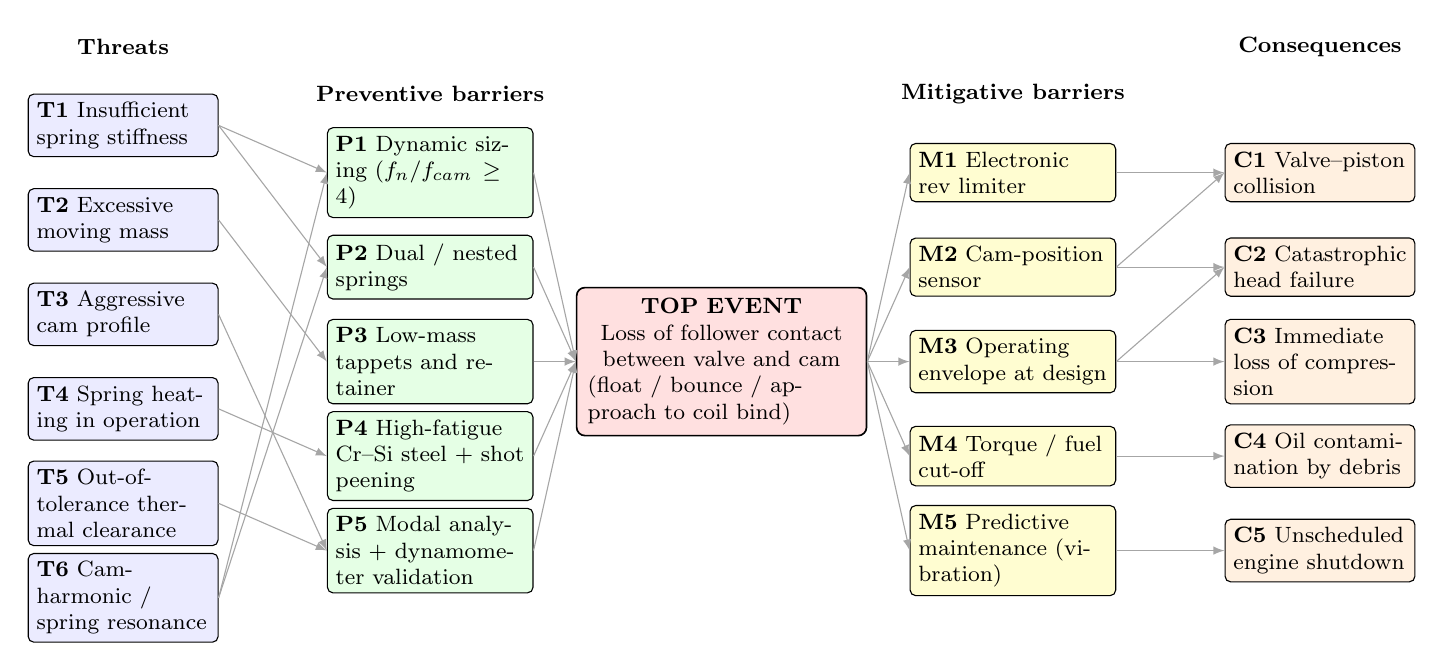
\begin{tikzpicture}[
  font=\footnotesize,
  every node/.style={align=left},
  threat/.style={draw,fill=blue!8,rounded corners=2pt,inner sep=3pt,minimum width=22mm,minimum height=6mm,text width=22mm},
  pbar/.style={draw,fill=green!10,rounded corners=2pt,inner sep=3pt,minimum width=24mm,minimum height=6mm,text width=24mm},
  cons/.style={draw,fill=orange!12,rounded corners=2pt,inner sep=3pt,minimum width=22mm,minimum height=6mm,text width=22mm},
  mbar/.style={draw,fill=yellow!18,rounded corners=2pt,inner sep=3pt,minimum width=24mm,minimum height=6mm,text width=24mm},
  topev/.style={draw,fill=red!12,line width=0.6pt,rounded corners=3pt,inner sep=4pt,minimum width=34mm,minimum height=12mm,text width=34mm},
  flow/.style={->,>=latex,line width=0.4pt,gray!70},
]

% ---- Top event (centre)
\node[topev] (TE) at (0,0)
  {\centering\textbf{TOP EVENT}\\Loss of follower contact between valve and cam\\(float / bounce / approach to coil bind)};

% ---- Threats (left, T1..T6)
\node[threat] (T1) at (-7.6, 3.0) {\textbf{T1} Insufficient spring stiffness};
\node[threat] (T2) at (-7.6, 1.8) {\textbf{T2} Excessive moving mass};
\node[threat] (T3) at (-7.6, 0.6) {\textbf{T3} Aggressive cam profile};
\node[threat] (T4) at (-7.6,-0.6) {\textbf{T4} Spring heating in operation};
\node[threat] (T5) at (-7.6,-1.8) {\textbf{T5} Out-of-tolerance thermal clearance};
\node[threat] (T6) at (-7.6,-3.0) {\textbf{T6} Cam-harmonic / spring resonance};

% ---- Preventive barriers (between threats and TE)
\node[pbar] (P1) at (-3.7, 2.4) {\textbf{P1} Dynamic sizing ($f_n/f_{cam}\geq 4$)};
\node[pbar] (P2) at (-3.7, 1.2) {\textbf{P2} Dual / nested springs};
\node[pbar] (P3) at (-3.7, 0.0) {\textbf{P3} Low-mass tappets and retainer};
\node[pbar] (P4) at (-3.7,-1.2) {\textbf{P4} High-fatigue Cr--Si steel + shot peening};
\node[pbar] (P5) at (-3.7,-2.4) {\textbf{P5} Modal analysis + dynamometer validation};

% ---- Consequences (right, C1..C5)
\node[cons] (C1) at (7.6, 2.4) {\textbf{C1} Valve--piston collision};
\node[cons] (C2) at (7.6, 1.2) {\textbf{C2} Catastrophic head failure};
\node[cons] (C3) at (7.6, 0.0) {\textbf{C3} Immediate loss of compression};
\node[cons] (C4) at (7.6,-1.2) {\textbf{C4} Oil contamination by debris};
\node[cons] (C5) at (7.6,-2.4) {\textbf{C5} Unscheduled engine shutdown};

% ---- Mitigative barriers (between TE and consequences)
\node[mbar] (M1) at (3.7, 2.4) {\textbf{M1} Electronic rev limiter};
\node[mbar] (M2) at (3.7, 1.2) {\textbf{M2} Cam-position sensor};
\node[mbar] (M3) at (3.7, 0.0) {\textbf{M3} Operating envelope at design};
\node[mbar] (M4) at (3.7,-1.2) {\textbf{M4} Torque / fuel cut-off};
\node[mbar] (M5) at (3.7,-2.4) {\textbf{M5} Predictive maintenance (vibration)};

% ---- Threats -> Preventive barriers (many-to-some mapping)
\draw[flow] (T1.east) -- (P1.west);
\draw[flow] (T2.east) -- (P3.west);
\draw[flow] (T3.east) -- (P5.west);
\draw[flow] (T4.east) -- (P4.west);
\draw[flow] (T5.east) -- (P5.west);
\draw[flow] (T6.east) -- (P1.west);
\draw[flow] (T1.east) -- (P2.west);
\draw[flow] (T6.east) -- (P2.west);

% ---- Preventive barriers -> Top event
\draw[flow] (P1.east) -- (TE.west);
\draw[flow] (P2.east) -- (TE.west);
\draw[flow] (P3.east) -- (TE.west);
\draw[flow] (P4.east) -- (TE.west);
\draw[flow] (P5.east) -- (TE.west);

% ---- Top event -> Mitigative barriers
\draw[flow] (TE.east) -- (M1.west);
\draw[flow] (TE.east) -- (M2.west);
\draw[flow] (TE.east) -- (M3.west);
\draw[flow] (TE.east) -- (M4.west);
\draw[flow] (TE.east) -- (M5.west);

% ---- Mitigative barriers -> Consequences
\draw[flow] (M1.east) -- (C1.west);
\draw[flow] (M2.east) -- (C1.west);
\draw[flow] (M3.east) -- (C2.west);
\draw[flow] (M3.east) -- (C3.west);
\draw[flow] (M4.east) -- (C4.west);
\draw[flow] (M5.east) -- (C5.west);
\draw[flow] (M2.east) -- (C2.west);

% ---- Side labels
\node[font=\footnotesize\bfseries] at (-7.6, 4.0) {Threats};
\node[font=\footnotesize\bfseries] at (-3.7, 3.4) {Preventive barriers};
\node[font=\footnotesize\bfseries] at ( 3.7, 3.4) {Mitigative barriers};
\node[font=\footnotesize\bfseries] at ( 7.6, 4.0) {Consequences};

\end{tikzpicture}

  \caption{BowTie diagram of the valve train of the AP 1.8 cylinder head operating at 10\,000~rpm. Threats (T1--T6) and preventive barriers (P1--P5) are arranged on the left side; consequences (C1--C5) and mitigative barriers (M1--M5) are arranged on the right side. The top event is the loss of follower contact between the valve and the cam, which encompasses valve float, valve bounce, and approach to coil bind.}\label{fig:bowtie}
\end{figure*}

% ----------------------------------------------------------------------
\subsection{Quantitative evaluation of the preventive barriers}
\label{sec:res-quant}

The five quantitative indicators of Table~\ref{tbl:quant-criteria} were
evaluated for the AP 1.8 head under the operating envelope of
Table~\ref{tbl:premises}. The numerical results are reported in
Table~\ref{tbl:quant-results} and discussed below.

% ----------------------------------------------------------------------
\paragraph{Dynamic follower contact.}
At the critical deceleration point of the cam ($a_{\max,-}=20\,362$~m\,s$^{-2}$,
$L_{-}=8.747$~mm), the spring force is
\begin{equation}
F_{\mathrm{spring},-}=F_{\mathrm{seat}}+k_{\mathrm{total}}\,L_{-}=780+99.49\times 8.747=1\,650.2~\mathrm{N},
\label{eq:Fspring}
\end{equation}
and the inertial force on the intake side, computed with the direct
translational mass of $43.48$~g, is
$F_{i,d,-,\mathrm{adm}}=885.3$~N, giving a dynamic ratio of
$R_{d,-,\mathrm{adm}}=1.864$. With the equivalent mass that includes
the reflected rocker (\,$49.59$~g\,), the dynamic ratio decreases to
$R_{\mathrm{eq},-,\mathrm{adm}}=1.634$. On the exhaust side, the larger
mass ($54.25$~g translational direct) yields
$R_{d,-,\mathrm{esc}}=1.494$ and $R_{\mathrm{eq},-,\mathrm{esc}}=1.343$.
All four values are above the $R\geq 1.20$ project criterion, so the
follower-contact barrier is satisfied with a margin of at least
12\,\% (in the worst case, the exhaust side with reflected rocker).

% ----------------------------------------------------------------------
\paragraph{Spring natural frequency.}
The fundamental surge mode of a helical compression spring with both
ends fixed is the first axial standing wave on the helical wire. For
a spring of stiffness $k$ and active mass $m_{s}$, the wave equation
yields a fundamental frequency
$\omega_{1}=\pi\sqrt{k/m_{s}}$~rad\,s$^{-1}$, hence
$f_{n}=\omega_{1}/(2\pi)=\tfrac{1}{2}\sqrt{k/m_{s}}$~Hz, which is the
form given in \citet[Eq.~10-26]{shigley2020}. This expression is
algebraically equivalent to the continuous-medium derivation
$f_{n}=(d/(2\pi N D_{m}^{2}))\sqrt{G/(2\rho)}$ of
\citet[\S~6.6]{heywood1988}: substituting
$k=Gd^{4}/(8 D_{m}^{3} N)$ and the active-coil wire mass
$m_{s}=(\pi^{2}/4)\,N D_{m} d^{2} \rho$ in
$f_{n}=\tfrac{1}{2}\sqrt{k/m_{s}}$ recovers Heywood's expression
exactly. In the present analysis the conservative lower bound is
adopted by using the \emph{total} spring mass (94.34~g for the outer
and 47.11~g for the inner spring), which includes the inactive end
turns and yields the lower bound of the surge frequency:
\begin{align}
f_{n,\mathrm{out}}&=\tfrac{1}{2}\sqrt{38\,060~\mathrm{N\,m^{-1}}/0.09434~\mathrm{kg}}\approx 318~\mathrm{Hz},\label{eq:fn-out}\\
f_{n,\mathrm{in}} &=\tfrac{1}{2}\sqrt{61\,430~\mathrm{N\,m^{-1}}/0.04711~\mathrm{kg}}\approx 571~\mathrm{Hz}.\label{eq:fn-in}
\end{align}
For comparison, replacing $m_{s,\mathrm{total}}$ with the conventional
effective mass $m_{s}/3$ (Rayleigh's quotient for a uniform coil
spring with one end fixed) would yield $f_{n,\mathrm{out}}\approx
551$~Hz and $f_{n,\mathrm{in}}\approx 988$~Hz. Adopting the total
spring mass therefore penalises the rule-of-thumb test against the
cam harmonics by a factor of $\sqrt{3}\approx 1.73$ and is treated
here as an explicit robustness check rather than a tolerance estimate.
The camshaft fundamental frequency at 10\,000~rpm engine speed
($f_{\mathrm{cam,max}}=10\,000/(2\times 60)=83.3$~Hz, the factor
two accounting for the 4-stroke cam-to-engine speed ratio) gives
the natural-frequency margins
$f_{n,\mathrm{out}}/f_{\mathrm{cam,max}}\approx 3.81$ and
$f_{n,\mathrm{in}}/f_{\mathrm{cam,max}}\approx 6.85$. The outer
spring sits just below the conventional
$f_{n}/f_{\mathrm{cam}}\geq 4$ threshold \citep{heywood1988} and is
therefore at the limit of the preventive barrier; the inner spring
is comfortably above the threshold against the cam fundamental.
However, real cam profiles contain harmonic content up to the sixth
to eighth harmonic, and the proximity of $f_{n,\mathrm{in}}\approx
571$~Hz to the sixth harmonic
($6\,f_{\mathrm{cam,max}}=500$~Hz; about 14\,\% separation) is
discussed in Section~\ref{sec:res-curves} and noted as a residual
concern.

% ----------------------------------------------------------------------
\paragraph{Coil-bind margin.}
At the maximum valve lift of 12.12~mm, the outer spring is compressed
to a height of $H_{\mathrm{open}}=34.38$~mm. With a solid height of
$H_{\mathrm{cb,out}}\approx 33.6$~mm (from $N_{t,\mathrm{out}}\,d_{\mathrm{out}}$),
the residual margin to coil bind is
\begin{equation}
M_{\mathrm{out}}=H_{\mathrm{open}}-H_{\mathrm{cb,out}}=34.38-33.6=0.78~\mathrm{mm},
\label{eq:Mout}
\end{equation}
which is below the project specification of $M\geq 1.5$~mm at
10\,000~rpm. In the concentric dual-spring assembly the inner and
outer springs share the same retainer and therefore undergo the same
axial compression at full lift, so $H_{\mathrm{open}}$ is identical
for both. The inner spring, with $H_{\mathrm{cb,in}}\approx 32.0$~mm,
therefore yields $M_{\mathrm{in}}=H_{\mathrm{open}}-H_{\mathrm{cb,in}}=34.38-32.0=2.38$~mm,
comfortably above the criterion. The
outer-spring coil-bind margin is therefore the only barrier that does
not satisfy its pass criterion under the current configuration of the
AP 1.8 head.

% ----------------------------------------------------------------------
\paragraph{Fatigue stress.}
The peak shear stress at full lift, computed with the Wahl-corrected
formula $\tau_{\max}=K_{w}\,8FD_{m}/(\pi d^{3})$, is
$\tau_{\mathrm{out}}\approx 655$~MPa for the outer spring
($K_{w,\mathrm{out}}=1.239$, $D_{m,\mathrm{out}}=30.2$~mm,
$d_{\mathrm{out}}=4.8$~mm) and $\tau_{\mathrm{in}}\approx 1\,232$~MPa
for the inner spring ($K_{w,\mathrm{in}}=1.329$,
$D_{m,\mathrm{in}}=19.0$~mm, $d_{\mathrm{in}}=4.0$~mm). Because the
spring operates between a non-zero seat preload and the full-lift
load, the proper criterion is the alternating-mean Goodman criterion
\citep[\S~10-7]{shigley2020} rather than a single-point comparison
with an allowable. With the corresponding seat-load shear stresses
$\tau_{\mathrm{out},\mathrm{seat}}\approx 257$~MPa and
$\tau_{\mathrm{in},\mathrm{seat}}\approx 484$~MPa, the alternating
and mean components are
$\tau_{a,\mathrm{out}}=199$~MPa, $\tau_{m,\mathrm{out}}=456$~MPa
and $\tau_{a,\mathrm{in}}=374$~MPa, $\tau_{m,\mathrm{in}}=858$~MPa.

For shot-peened ASTM~A877/A877M chrome--silicon valve-spring steel,
typical strengths are an ultimate tensile strength
$S_{ut}\approx 1\,900$~MPa, an ultimate shear strength
$S_{su}\approx 0.67\,S_{ut}\approx 1\,270$~MPa, and a shear endurance
limit after shot peening and surface control of
$S_{se}\approx 465$~MPa
\citep[\S~10-30]{shigley2020}. The Goodman factor of safety is then
\begin{equation}
\frac{1}{n_{f}}=\frac{\tau_{a}}{S_{se}}+\frac{\tau_{m}}{S_{su}}.
\label{eq:goodman}
\end{equation}
For the outer spring this gives
$1/n_{f,\mathrm{out}}=199/465+456/1\,270\approx 0.428+0.359=0.787$,
hence $n_{f,\mathrm{out}}\approx 1.27$ (active, with positive but
not generous margin). For the inner spring,
$1/n_{f,\mathrm{in}}=374/465+858/1\,270\approx 0.804+0.676=1.480$,
hence $n_{f,\mathrm{in}}\approx 0.68$, which is below unity and
indicates that the baseline configuration of the inner spring does
not satisfy the Goodman criterion. The inner-spring fatigue barrier
is therefore reclassified as \textbf{at risk} in
Table~\ref{tbl:quant-results}, alongside the outer-spring coil-bind
margin. This finding is consistent with
\citet{xing2021valvespringEAC,ko2022springfatigueflaws}, who report
that small surface flaws and environment-assisted cracking
substantially reduce the fatigue life of high-strength valve springs
loaded close to their nominal allowable.

% ----------------------------------------------------------------------
\paragraph{Hot clearance.}
A complete thermal expansion model of the cylinder head and valve
train is outside the scope of the present study, but a first-order
estimate of the magnitude can be obtained from the linear thermal
expansion of the longest element of the train, the exhaust valve stem
(length $L_{h}=180$~mm, INCONEL 751 with
$\alpha\approx 13\times 10^{-6}~\mathrm{K}^{-1}$). For an exhaust-side
temperature rise of $\Delta T\approx 600$~K above the cold-assembly
condition, the stem elongates by
$\Delta L = \alpha L_{h} \Delta T \approx 1.4$~mm. The corresponding
cold mechanical clearance must therefore be at least
$\sim$1.5~mm to maintain a positive hot clearance, a value compatible
with the design clearance typically specified for high-rpm performance
heads \citep{heisler2002}. This worst-case estimate neglects the
thermal expansion of the aluminium cylinder head, which acts in the
opposite sense and partially compensates the valve-stem elongation;
including it would relax the cold-clearance requirement. A dedicated
differential thermal-mechanical analysis is left for future work and
listed in the Limitations of Section~\ref{sec:disc-limitations}.

% ----------------------------------------------------------------------
% Consolidated table
% ----------------------------------------------------------------------
\begin{table*}[width=\textwidth,cols=4,pos=t]
\caption{Quantitative results for the five preventive barriers of the BowTie diagram applied to the AP 1.8 valve train at 10\,000~rpm. Values traced to the sizing of the intake valve and the valve springs.}\label{tbl:quant-results}
\begin{tabular*}{\tblwidth}{@{}LCCC@{}}
\toprule
Barrier & Indicator & Value & Status \\
\midrule
Dynamic follower contact (intake, direct mass) & $R_{d,-,\mathrm{adm}}$ & 1.864 & active ($\geq 1.20$) \\
Dynamic follower contact (intake, with rocker) & $R_{\mathrm{eq},-,\mathrm{adm}}$ & 1.634 & active ($\geq 1.20$) \\
Dynamic follower contact (exhaust, direct mass) & $R_{d,-,\mathrm{esc}}$ & 1.494 & active ($\geq 1.20$) \\
Dynamic follower contact (exhaust, with rocker) & $R_{\mathrm{eq},-,\mathrm{esc}}$ & 1.343 & active ($\geq 1.20$) \\
Natural frequency (outer spring) & $f_{n,\mathrm{out}}/f_{\mathrm{cam,max}}$ & 3.81 & at limit ($<4$) \\
Natural frequency (inner spring) & $f_{n,\mathrm{in}}/f_{\mathrm{cam,max}}$ & 6.85 & active ($\geq 4$) \\
Coil-bind margin (outer spring) & $M_{\mathrm{out}}$ & 0.78~mm & \textbf{at risk} ($<1.5$~mm) \\
Coil-bind margin (inner spring) & $M_{\mathrm{in}}$ & 2.38~mm & active ($\geq 1.5$~mm) \\
Fatigue Goodman FoS (outer spring) & $n_{f,\mathrm{out}}$ & 1.27 & active ($\geq 1$) \\
Fatigue Goodman FoS (inner spring) & $n_{f,\mathrm{in}}$ & 0.68 & \textbf{at risk} ($<1$) \\
Hot clearance$^{\dagger}$ & $c(T_{\max})$ & --- & qualitatively verified (see Sec.~\ref{sec:res-quant}) \\
\bottomrule
\end{tabular*}
{\footnotesize $^{\dagger}$Outside the deterministic layer; only a first-order order-of-magnitude estimate is reported.}
\end{table*}

% ----------------------------------------------------------------------
\subsection{Critical-barrier identification}\label{sec:res-critical}

A tornado plot of the sensitivity of each indicator to its dominant
input is shown in Fig.~\ref{fig:tornado}. For each barrier, the input
perturbed by $\pm$10\,\% is the dominant parameter governing the
indicator: the spring stiffness $k$ for the natural-frequency margin,
the maximum cam lift $L_{\mathrm{cam}}^{\max}$ for the coil-bind
margin, the moving mass $m$ for the dynamic-ratio margin, and the
shear-stress amplitude $\tau_{a}$ for the Goodman fatigue margin. The
$\pm$10\,\% perturbation is adopted as a uniform stress test rather
than a tolerance estimate, providing an upper-bound sensitivity
envelope for the worst-case parameter drift. The actual ASTM~A877/A877M
specification tolerances are tighter and unequal by parameter
(typically $\pm$1.5\,\% on free length, $\pm$0.5\,\% on wire diameter,
and $\pm$3\,\% on shear modulus); a refined sensitivity analysis based
on those non-uniform tolerances is identified as future work. The bar length
corresponds to the absolute change in the residual margin under that
perturbation. The analysis identifies \textbf{three} barriers as
exposed to parametric drift: the \emph{outer-spring coil-bind margin}
($M_{\mathrm{out}}=0.78$~mm, violating its pass criterion already in
the baseline configuration), the \emph{inner-spring fatigue Goodman
factor of safety}
($n_{f,\mathrm{in}}=0.68$, below unity in the baseline configuration),
and the \emph{outer-spring natural-frequency margin}
($f_{n,\mathrm{out}}/f_{\mathrm{cam,max}}=3.81$, just below the
conventional 4$\times$ rule of thumb).

The findings indicate that the AP 1.8 dual-spring assembly has
\emph{two} concurrent at-risk barriers in the baseline configuration:
the outer-spring coil-bind margin and the inner-spring fatigue
factor of safety. They are not redundant: they affect different
springs (outer vs inner) and act through different physical
mechanisms (geometric clearance vs cyclic shear loading). The
outer-spring natural-frequency margin sits just below the
conventional threshold and is treated as a residual concern. The
sizing note for the springs already prescribes the geometric
correction for the outer-spring coil-bind --- raising the installed
height to $H_{\mathrm{inst,ideal}}=47.72$~mm and the free length to
$L_{0,\mathrm{ideal}}=55.56$~mm to recover an $M\approx 2.0$~mm
margin. The inner-spring fatigue concern is not addressed by that
geometric change and would require a different intervention:
increasing the wire diameter $d_{\mathrm{in}}$, reducing the spring
index $C_{\mathrm{in}}=D_{m,\mathrm{in}}/d_{\mathrm{in}}$, or
adopting a higher-grade chrome--silicon--vanadium steel with a
larger shear endurance limit. The two findings together reinforce
the value of the quantitative-coupled BowTie approach: a single-point
comparison of $\tau_{\max}$ with an upper-bound allowable, in the
spirit of conventional FMEA, would have classified the inner-spring
fatigue as nominally acceptable, whereas the Goodman criterion
exposes the deficit unambiguously.

\begin{figure}[t]
  \centering
  \resizebox{\linewidth}{!}{% =====================================================================
% Figure 4 — Tornado plot (TikZ-native, manual bars)
% Each bar shows the residual margin of one preventive-barrier indicator
% as a percentage above the pass criterion. Negative = barrier violated.
% =====================================================================

\begin{tikzpicture}[
  font=\footnotesize,
  bar/.style={fill=blue!45, draw=blue!60!black, line width=0.4pt},
  barfail/.style={fill=red!55, draw=red!75!black, line width=0.4pt},
  bargrey/.style={fill=gray!35, draw=gray!60, line width=0.4pt, pattern=north east lines, pattern color=gray!50},
  axisline/.style={->,>=latex,line width=0.5pt},
  threshold/.style={red!75!black, line width=0.6pt, dashed},
]

% Geometry: axis spans -50% to +60% horizontally
% Each row: 0.55 cm tall, 7 rows total

% --- Axis
\def\xmin{-2.6}
\def\xmax{6.0}
\def\xscale{1.0}    % 1 cm = 10%
\draw[axisline] (\xmin,0) -- (\xmax+0.4,0)
  node[anchor=west, font=\footnotesize] {Margin (\%)};

% Tick marks every 20%
\foreach \x in {-40,-20,0,20,40,60} {
  \pgfmathsetmacro{\xpos}{\x/10}
  \draw (\xpos,-0.1) -- (\xpos,0.1) node[below=4pt, font=\scriptsize] {\x};
}

% --- Vertical pass-threshold line at 0
\draw[threshold] (0,-0.3) -- (0,4.6);
\node[red!75!black, font=\scriptsize, anchor=south] at (0, 4.6) {pass};

% --- Bars (top to bottom)
% Row positions:  4.0, 3.4, 2.8, 2.2, 1.6, 1.0, 0.4

% Row 1: R_eq,-,esc = +11.9% (active)
\fill[bar] (0,3.85) rectangle (1.19,4.15);
\node[anchor=east, font=\footnotesize] at (\xmin,4.0)
  {$R_{\mathrm{eq},-,\mathrm{esc}}$ (follower)};
\node[anchor=west, font=\scriptsize] at (1.25,4.0) {$+11.9\%$};

% Row 2: f_n,out/f_cam = -4.8% (at limit)
\fill[barfail] (-0.48,3.25) rectangle (0,3.55);
\node[anchor=east, font=\footnotesize] at (\xmin,3.4)
  {$f_{n,\mathrm{out}}/f_{\mathrm{cam}}$ (surge)};
\node[anchor=east, font=\scriptsize] at (-0.55,3.4) {$-4.8\%$};

% Row 3: M_out = -48% (FAIL, critical barrier — value annotation includes [critical])
\fill[barfail] (-2.6,2.65) rectangle (0,2.95);
\node[anchor=east, font=\footnotesize] at (\xmin,2.8)
  {$M_{\mathrm{out}}$ (coil bind, outer)};
\node[anchor=west, font=\footnotesize, red!75!black] at (0.05,2.8)
  {$-48.0\%$ \,---\, critical};

% Row 4: M_in = +58.7% (active, comfortable)
\fill[bar] (0,2.05) rectangle (5.87,2.35);
\node[anchor=east, font=\footnotesize] at (\xmin,2.2)
  {$M_{\mathrm{in}}$ (coil bind, inner)};
\node[anchor=west, font=\scriptsize] at (5.95,2.2) {$+58.7\%$};

% Row 5: tau_out = +40.5%
\fill[bar] (0,1.45) rectangle (4.05,1.75);
\node[anchor=east, font=\footnotesize] at (\xmin,1.6)
  {$\tau_{\mathrm{out}}$ (fatigue, outer)};
\node[anchor=west, font=\scriptsize] at (4.10,1.6) {$+40.5\%$};

% Row 6: n_f,in (Goodman fatigue inner) = -32% (FAIL — at risk)
\fill[barfail] (-2.6,0.85) rectangle (0,1.15);
\node[anchor=east, font=\footnotesize] at (\xmin,1.0)
  {$n_{f,\mathrm{in}}$ (Goodman, inner)};
\node[anchor=west, font=\footnotesize, red!75!black] at (0.05,1.0)
  {$-32.0\%$ \,---\, at risk};

% Row 7: Hot clearance — not quantitatively assessed (gray hatched bar)
\fill[bargrey] (0,0.25) rectangle (1.0,0.55);
\node[anchor=east, font=\footnotesize] at (\xmin,0.4)
  {Hot clearance};
\node[anchor=west, font=\scriptsize] at (1.05,0.4) {n.a.};

\end{tikzpicture}
}
  \caption{Tornado plot of the sensitivity of each preventive-barrier indicator to its dominant input under a $\pm$10\,\% perturbation. Two indicators (in red) violate their pass criteria already in the baseline configuration and are identified as critical preventive barriers of the AP 1.8 valve train at 10\,000~rpm: the outer-spring coil-bind margin $M_{\mathrm{out}}$ ($-48.0\%$) and the inner-spring fatigue Goodman factor of safety $n_{f,\mathrm{in}}$ ($-32.0\%$). The outer-spring natural-frequency margin $f_{n,\mathrm{out}}/f_{\mathrm{cam,max}}$ ($-4.8\%$) sits just below the conventional 4$\times$ rule-of-thumb threshold and is treated separately as a residual concern.}\label{fig:tornado}
\end{figure}

% ----------------------------------------------------------------------
\subsection{Lift profile and natural-frequency map}
\label{sec:res-curves}

For completeness, Fig.~\ref{fig:lift} shows the position of the two
critical points of the cam profile (positive-acceleration peak and
deceleration peak) on the lift--versus--crank-angle plane;
Fig.~\ref{fig:fn} compares the spring natural frequencies with the
first cam harmonics across the rotational-speed range up to
10\,000~rpm engine speed.

\begin{figure}[t]
  \centering
  % =====================================================================
% Figure 2 — Cam lift schematic (TikZ + pgfplots)
% Shows the two critical points of the cam profile (positive accel
% peak and deceleration peak), reconstructed analytically from the
% cam dimensioning of the AP 1.8 head.
% =====================================================================

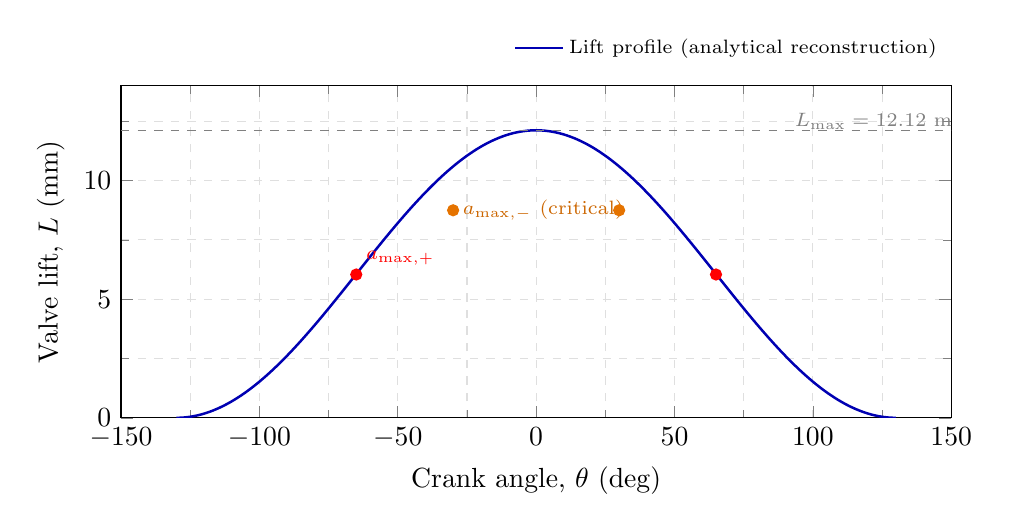
\begin{tikzpicture}
  \begin{axis}[
    width=\linewidth,
    height=5.8cm,
    xlabel={Crank angle, $\theta$ (deg)},
    ylabel={Valve lift, $L$ (mm)},
    xmin=-150, xmax=150,
    ymin=0,    ymax=14,
    grid=both,
    grid style={dashed,gray!25},
    minor tick num=1,
    legend style={
      at={(1,1.05)}, anchor=south east,
      font=\scriptsize, draw=none, fill=none,
      legend columns=-1,
    },
  ]
  % Smooth bell-shaped lift curve (analytical reconstruction).
  % Peak lift L_max = 12.12 mm at theta = 0 deg.
  \addplot[blue!70!black, line width=0.9pt, smooth, samples=200, domain=-130:130]
    {12.12 * (cos(deg(pi*x/260)))^2};
  \addlegendentry{Lift profile (analytical reconstruction)}

  % Critical point 1: positive acceleration peak (L+ = 6.04 mm)
  \addplot[red, mark=*, mark size=2.0pt, only marks] coordinates {(-65, 6.04)};
  \node[anchor=south west, red, font=\scriptsize] at (axis cs:-65,6.04) {$a_{\max,+}$};

  % Critical point 2: deceleration peak (L- = 8.747 mm)
  \addplot[orange!90!black, mark=*, mark size=2.0pt, only marks] coordinates {(-30, 8.747)};
  \node[anchor=west, orange!80!black, font=\scriptsize] at (axis cs:-30,8.747) {$a_{\max,-}$ (critical)};

  % Symmetric points on closing side
  \addplot[red,        mark=*, mark size=2.0pt, only marks] coordinates {( 65, 6.04)};
  \addplot[orange!90!black, mark=*, mark size=2.0pt, only marks] coordinates {( 30, 8.747)};

  % L_max line
  \addplot[gray, dashed] coordinates {(-150,12.12) (150,12.12)};
  \node[anchor=west, gray, font=\scriptsize] at (axis cs:90,12.5) {$L_{\max}=12.12$ mm};

  \end{axis}
\end{tikzpicture}

  \caption{Schematic position of the two critical points of the cam profile of the AP 1.8 high-performance head: positive-acceleration peak ($a_{\max,+}=14\,544$~m\,s$^{-2}$ at $L_{+}=6.04$~mm) and deceleration peak ($a_{\max,-}=20\,362$~m\,s$^{-2}$ at $L_{-}=8.747$~mm). The full lift profile is generated from the cam sizing of the intake valve.}\label{fig:lift}
\end{figure}

\begin{figure}[t]
  \centering
  \resizebox{\linewidth}{!}{% =====================================================================
% Figure 3 — Spring natural frequency vs. cam harmonics (pgfplots)
% Shows f_{n,out} ≈ 318 Hz and f_{n,in} ≈ 571 Hz against the first
% six cam harmonics (n=1..6) over the engine speed range 0..10 000 rpm.
% Cam runs at half engine speed (4-stroke).
% =====================================================================

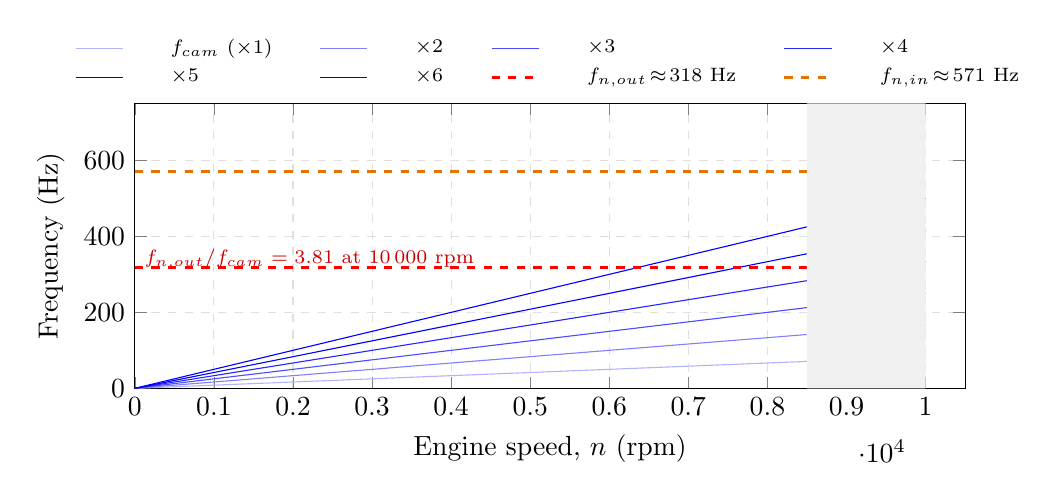
\begin{tikzpicture}
  \begin{axis}[
    width=\linewidth,
    height=5.2cm,
    xlabel={Engine speed, $n$ (rpm)},
    ylabel={Frequency (Hz)},
    xmin=0, xmax=10500,
    ymin=0, ymax=750,
    grid=both,
    grid style={dashed,gray!25},
    legend style={
      at={(0.5,1.02)}, anchor=south,
      legend columns=4,
      font=\scriptsize, draw=none, fill=none,
      column sep=1.5em,
      /tikz/every even column/.append style={column sep=1.5em},
    },
    legend cell align=left,
  ]
  % Cam harmonics: f_h(n) = h * (n_engine / 120). At 10000 rpm: 1*=83.3, 2*=166.7, 3*=250, 4*=333.3, 5*=416.7, 6*=500
  \addplot[domain=0:10000, samples=2, blue!30 ] {x/120};         \addlegendentry{$f_{cam}$ ($\times 1$)}
  \addplot[domain=0:10000, samples=2, blue!50 ] {2*x/120};       \addlegendentry{$\times 2$}
  \addplot[domain=0:10000, samples=2, blue!70 ] {3*x/120};       \addlegendentry{$\times 3$}
  \addplot[domain=0:10000, samples=2, blue!85 ] {4*x/120};       \addlegendentry{$\times 4$}
  \addplot[domain=0:10000, samples=2, blue!95!black] {5*x/120};  \addlegendentry{$\times 5$}
  \addplot[domain=0:10000, samples=2, blue!100!black] {6*x/120}; \addlegendentry{$\times 6$}

  % Spring natural frequencies (constant)
  \addplot[red, dashed, line width=0.9pt, domain=0:10000, samples=2] {318};
  \addlegendentry{$f_{n,out}\!\approx\!318$ Hz}
  \addplot[orange!90!black, dashed, line width=0.9pt, domain=0:10000, samples=2] {571};
  \addlegendentry{$f_{n,in}\!\approx\!571$ Hz}

  % Operating regime shading: 8500-10000 rpm
  \addplot[fill=gray!12, draw=none, forget plot] coordinates {(8500,0) (10000,0) (10000,750) (8500,750)} \closedcycle;

  % 4× rule-of-thumb threshold: 4 * f_cam at engine speed = f_n / 4
  % Annotation
  \node[anchor=west, red!80!black, font=\scriptsize] at (axis cs: 0, 340) {$f_{n,out}/f_{cam}=3.81$ at 10\,000 rpm};

  \end{axis}
\end{tikzpicture}
}
  \caption{Spring natural frequencies $f_{n,\mathrm{out}}$ and $f_{n,\mathrm{in}}$ compared with the first six cam harmonics ($n=1,\dots,6$) across the engine-speed range up to 10\,000~rpm. The shaded region marks the operating regime; the dashed horizontal lines mark $f_{n,\mathrm{out}}\approx 318$~Hz and $f_{n,\mathrm{in}}\approx 571$~Hz.}\label{fig:fn}
\end{figure}

% ----------------------------------------------------------------------
\subsection{Qualitative validation against documented failure cases}
\label{sec:res-litvalidation}

The deterministic indicators of
Table~\ref{tbl:quant-results} establish whether the AP 1.8 head
satisfies its design margins; they do not by themselves demonstrate
that the BowTie procedure would correctly flag the failure modes
encountered in service by other engines. To address that gap without
introducing experimental data that is not available for the AP 1.8
configuration, the four valve-train and engine-component failure
case studies catalogued in Table~\ref{tbl:related-cases} are now
re-examined as a qualitative validation set: each reported root
cause is matched with the BowTie barrier that, on the bow diagram of
Section~\ref{sec:res-bowtie}, would have been the controlling
element, and the deterministic indicator (if any) that would have
exposed the deficit at the design stage is identified. Four
outcomes are possible: \emph{caught on the deterministic side}
(a preventive-barrier indicator flags the deficit numerically),
\emph{caught on the mitigative side} (the failure mechanism is an
operational signature addressed by a mitigative barrier and outside
the preventive deterministic layer by construction),
\emph{flagged qualitatively only} (the threat is in the bow but no
quantitative indicator exists in the present formulation), or
\emph{outside the present scope} (the failure mechanism falls
outside the barrier set adopted here and would require an extension
of the procedure). The four cases populate all four outcomes.

\paragraph{\citet{xing2021valvespringEAC} --- caught on the
deterministic side.}
The premature fatigue of high-strength valve springs reported by
Xing is attributed to environment-assisted cracking, which depresses
the effective shear endurance limit $S_{se}$ below the catalogued
allowable for shot-peened wire. The preventive barrier P4
(\emph{high-fatigue-resistance spring material}) maps directly to
the Goodman factor of safety
$n_{f}$ of Eq.~\eqref{eq:goodman}, evaluated with a $S_{se}$
discounted for surface condition and lubricant chemistry as
recommended by the case study itself. In the present analysis the
discounted $S_{se}\approx 465$~MPa for shot-peened ASTM~A877/A877M
(see Section~\ref{sec:res-quant}, ``Fatigue stress'') is precisely
the value advocated by Xing. The fact that the same indicator,
applied to the AP 1.8 inner spring, returns
$n_{f,\mathrm{in}}\approx 0.68 < 1$ is the strongest demonstration
of the procedure: the indicator that diagnosed Xing's premature
failure at a generic level exposes the inner-spring deficit of the
AP 1.8 head before the prototype is built.

\paragraph{\citet{velezgodino2019overheadvalvetrain} --- caught on
the mitigative side.}
The recurrent in-service failure of the overhead valve train of
urban buses is attributed by V\'elez Godi\~no et al.\ to a
combination of operational misuse and inadequate inspection
intervals --- a maintenance and operational signature, not a
design-margin signature. By construction, this class of failure
falls on the mitigative side of the bow rather than on the
preventive side: barriers M3 (\emph{operating envelope defined at
design stage}) and M5 (\emph{predictive maintenance via vibration
signals}) are the controlling elements. The deterministic
indicators of Table~\ref{tbl:quant-criteria} would not have
flagged this case at the design stage --- and this is the correct
behaviour: the case is, by its own description, an operational
problem expressed at the maintenance interface. The BowTie diagram
visualises this distinction explicitly, whereas a single-score RPN
ranking blends preventive and mitigative dimensions into one number.

\paragraph{\citet{soffritti2018wornvalvetrain} --- flagged
qualitatively only.}
The premature wear at the rocker-arm/pushrod and rocker-arm/valve
interfaces in a four-cylinder diesel engine is attributed by
Soffritti et al.\ to valve misalignment with respect to the seat
insert. The threat ``out-of-tolerance assembly geometry'' is not
explicitly listed among $T_{1}$--$T_{6}$ in the bow of
Section~\ref{sec:method-bowtie-qual}, but it is a direct extension
of the existing threat structure: it sits next to $T_{2}$
(\emph{excessive moving mass}) and $T_{3}$
(\emph{aggressive cam profile}) as a geometric departure from the
sizing assumption. No deterministic indicator in
Table~\ref{tbl:quant-criteria} maps to it: the case is therefore
\emph{flagged qualitatively only} by the present procedure. This
outcome motivates a candidate extension of the preventive barrier
set --- an assembly/tolerance barrier $P_{6}$ with an indicator
based on the as-built valve-seat alignment --- which is identified
as a direction for future work in Section~\ref{sec:disc-limitations}.

\paragraph{\citet{zhao2023camshaftV6} --- outside the present
scope.}
The lubrication failure of the camshaft bearings of a V6 diesel
engine is attributed by Zhao et al.\ to an asperity-contact regime
that violates the design assumption of full hydrodynamic
lubrication. The present BowTie is centred on the spring--cam
dynamic interaction and does not include a lubrication-regime
preventive barrier; the case therefore lies outside the scope of
the procedure as formulated here. The honest outcome of the
comparison is that the procedure would have \emph{missed} this
failure mode --- and that explicit recognition is itself the
useful finding: an extension of the procedure with an additional
preventive barrier on the lubrication regime (e.g.\ a
Stribeck-curve-based indicator on the camshaft bearing pair) is
needed before the framework can claim coverage of the full set of
valve-train-related failure mechanisms.

\paragraph{Summary of the qualitative validation.}
Of the four documented case studies surveyed in
Table~\ref{tbl:related-cases}, one is caught quantitatively by the
deterministic indicator set (Xing, via the Goodman factor of
safety), one is caught on the mitigative side as designed
(V\'elez Godi\~no), one is flagged qualitatively but lies outside
the deterministic indicator set (Soffritti, motivating a candidate
$P_{6}$), and one is outside the present scope altogether (Zhao,
motivating a lubrication-regime extension). The pattern is
consistent: the procedure correctly distinguishes between
design-margin failures (where the deterministic indicators are
diagnostic), operational/maintenance failures (where the mitigative
side is diagnostic), and failure mechanisms outside the present
barrier set (where the comparison flags the limitation). This
qualitative validation supports the use of the procedure as a
design-stage check while confirming that an empirical campaign on
a dedicated test rig --- specified in Section~\ref{sec:conclusion}
--- remains necessary for quantitative validation of the indicator
margins reported here.
